\section{Circuit Implementation} \label{sec:implementation}
%\begin{figure} [!htbp]
%   \centering
%    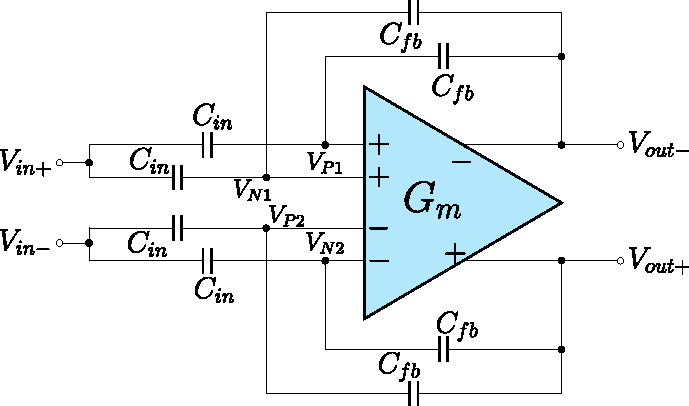
\includegraphics[width = 0.65\linewidth]{img/DL-CCIA.pdf}
%    \caption{ CCIA schematic with dual-loop architecture.}
%    \label{DLCCIA}
%\end{figure}


\begin{figure}[!h]
       \centering
       \begin{subfigure}[c]{0.49\linewidth}
           \centering
           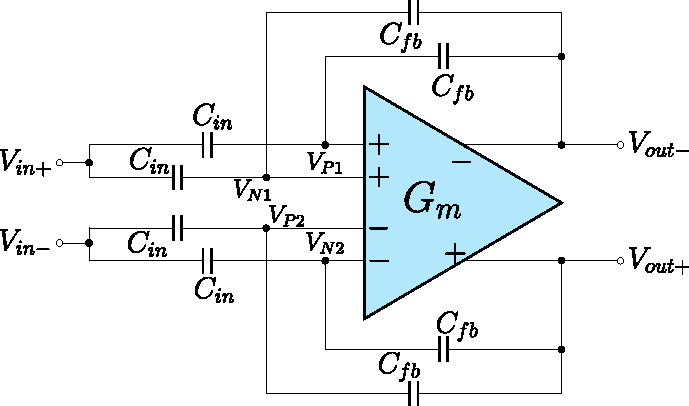
\includegraphics[width=\linewidth]{img/DL-CCIA.pdf}
           \caption[]%
           {{\small }}
           \label{fig:DL-CCIA}
        \end{subfigure}
        \hfill
        \begin{subfigure}[c]{0.45\linewidth}  
            \centering 
            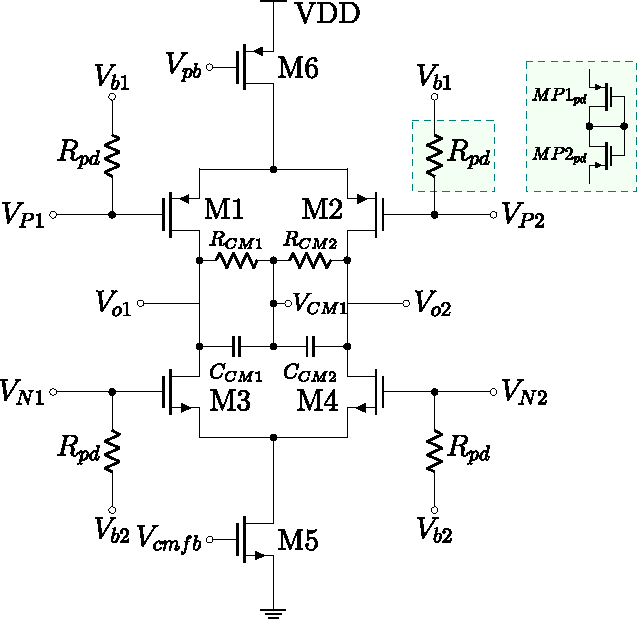
\includegraphics[width=\linewidth]{img/CurrentReuse.pdf}
            %\caption[5 DOF custom mount for MPFCS]%
            %{{\small 5 DOF custom mount for MPFCS}}    
            \caption[]%
            {{\small }}
            \label{fig:CRCI}
        \end{subfigure}
        \caption[ Don't write caption here ]
        {\small (a) CCIA schematic with dual-loop architecture. (b) Current-reuse amplifier schematic with individual biasing } 
        \label{fig:DL-CCIA and CRCI separate biasing}
\end{figure}

To validate the design methodology, a CCIA was designed in 65nm CMOS technology. Due to issues with gate leakage in this technology, thick oxide transistors were required for the current re-use input stage. A dual-loop CCIA (DL-CCIA) architecture as shown in \Cref{fig:DL-CCIA} was used to allow separate biasing of the input stages and achieve optimum $g_m/I_D$ for $V_{DD}=\SI{1.2}{\volt}$. The DL-CCIA was designed with an IRN requirement of $<\SI{2.5}{\nano\volt\per\sqrt{\hertz}}$. The \gmID values chosen for the PMOS and NMOS devices (see \cref{fig:CRCI}) were 18 and 17, respectively. The $L_P$ and $L_N$ were selected as 500nm and 700nm, respectively.  The gain of CCIA was set to $G=\SI{20}{\frac{\volt}{\volt}}$ to minimise the input referred noise of the PGA. From the area constraint, $C_{in}$ was \SI{11.6}{\pico\farad}.

